\documentclass{article}

\usepackage{graphicx}
\usepackage{tikz}
\usepackage{tikzsymbols}
\usetikzlibrary{calc,patterns,shapes.geometric}
\pagestyle{empty}
\usepackage[margin=0pt]{geometry}
\geometry{papersize={14in,12in}}

\def\centerarc[#1](#2)(#3:#4:#5){\draw[#1] ($(#2)+({#5*cos(#3)},{#5*sin(#3)})$) arc (#3:#4:#5);}

\begin{document}
	\begin{figure}
		\centering
		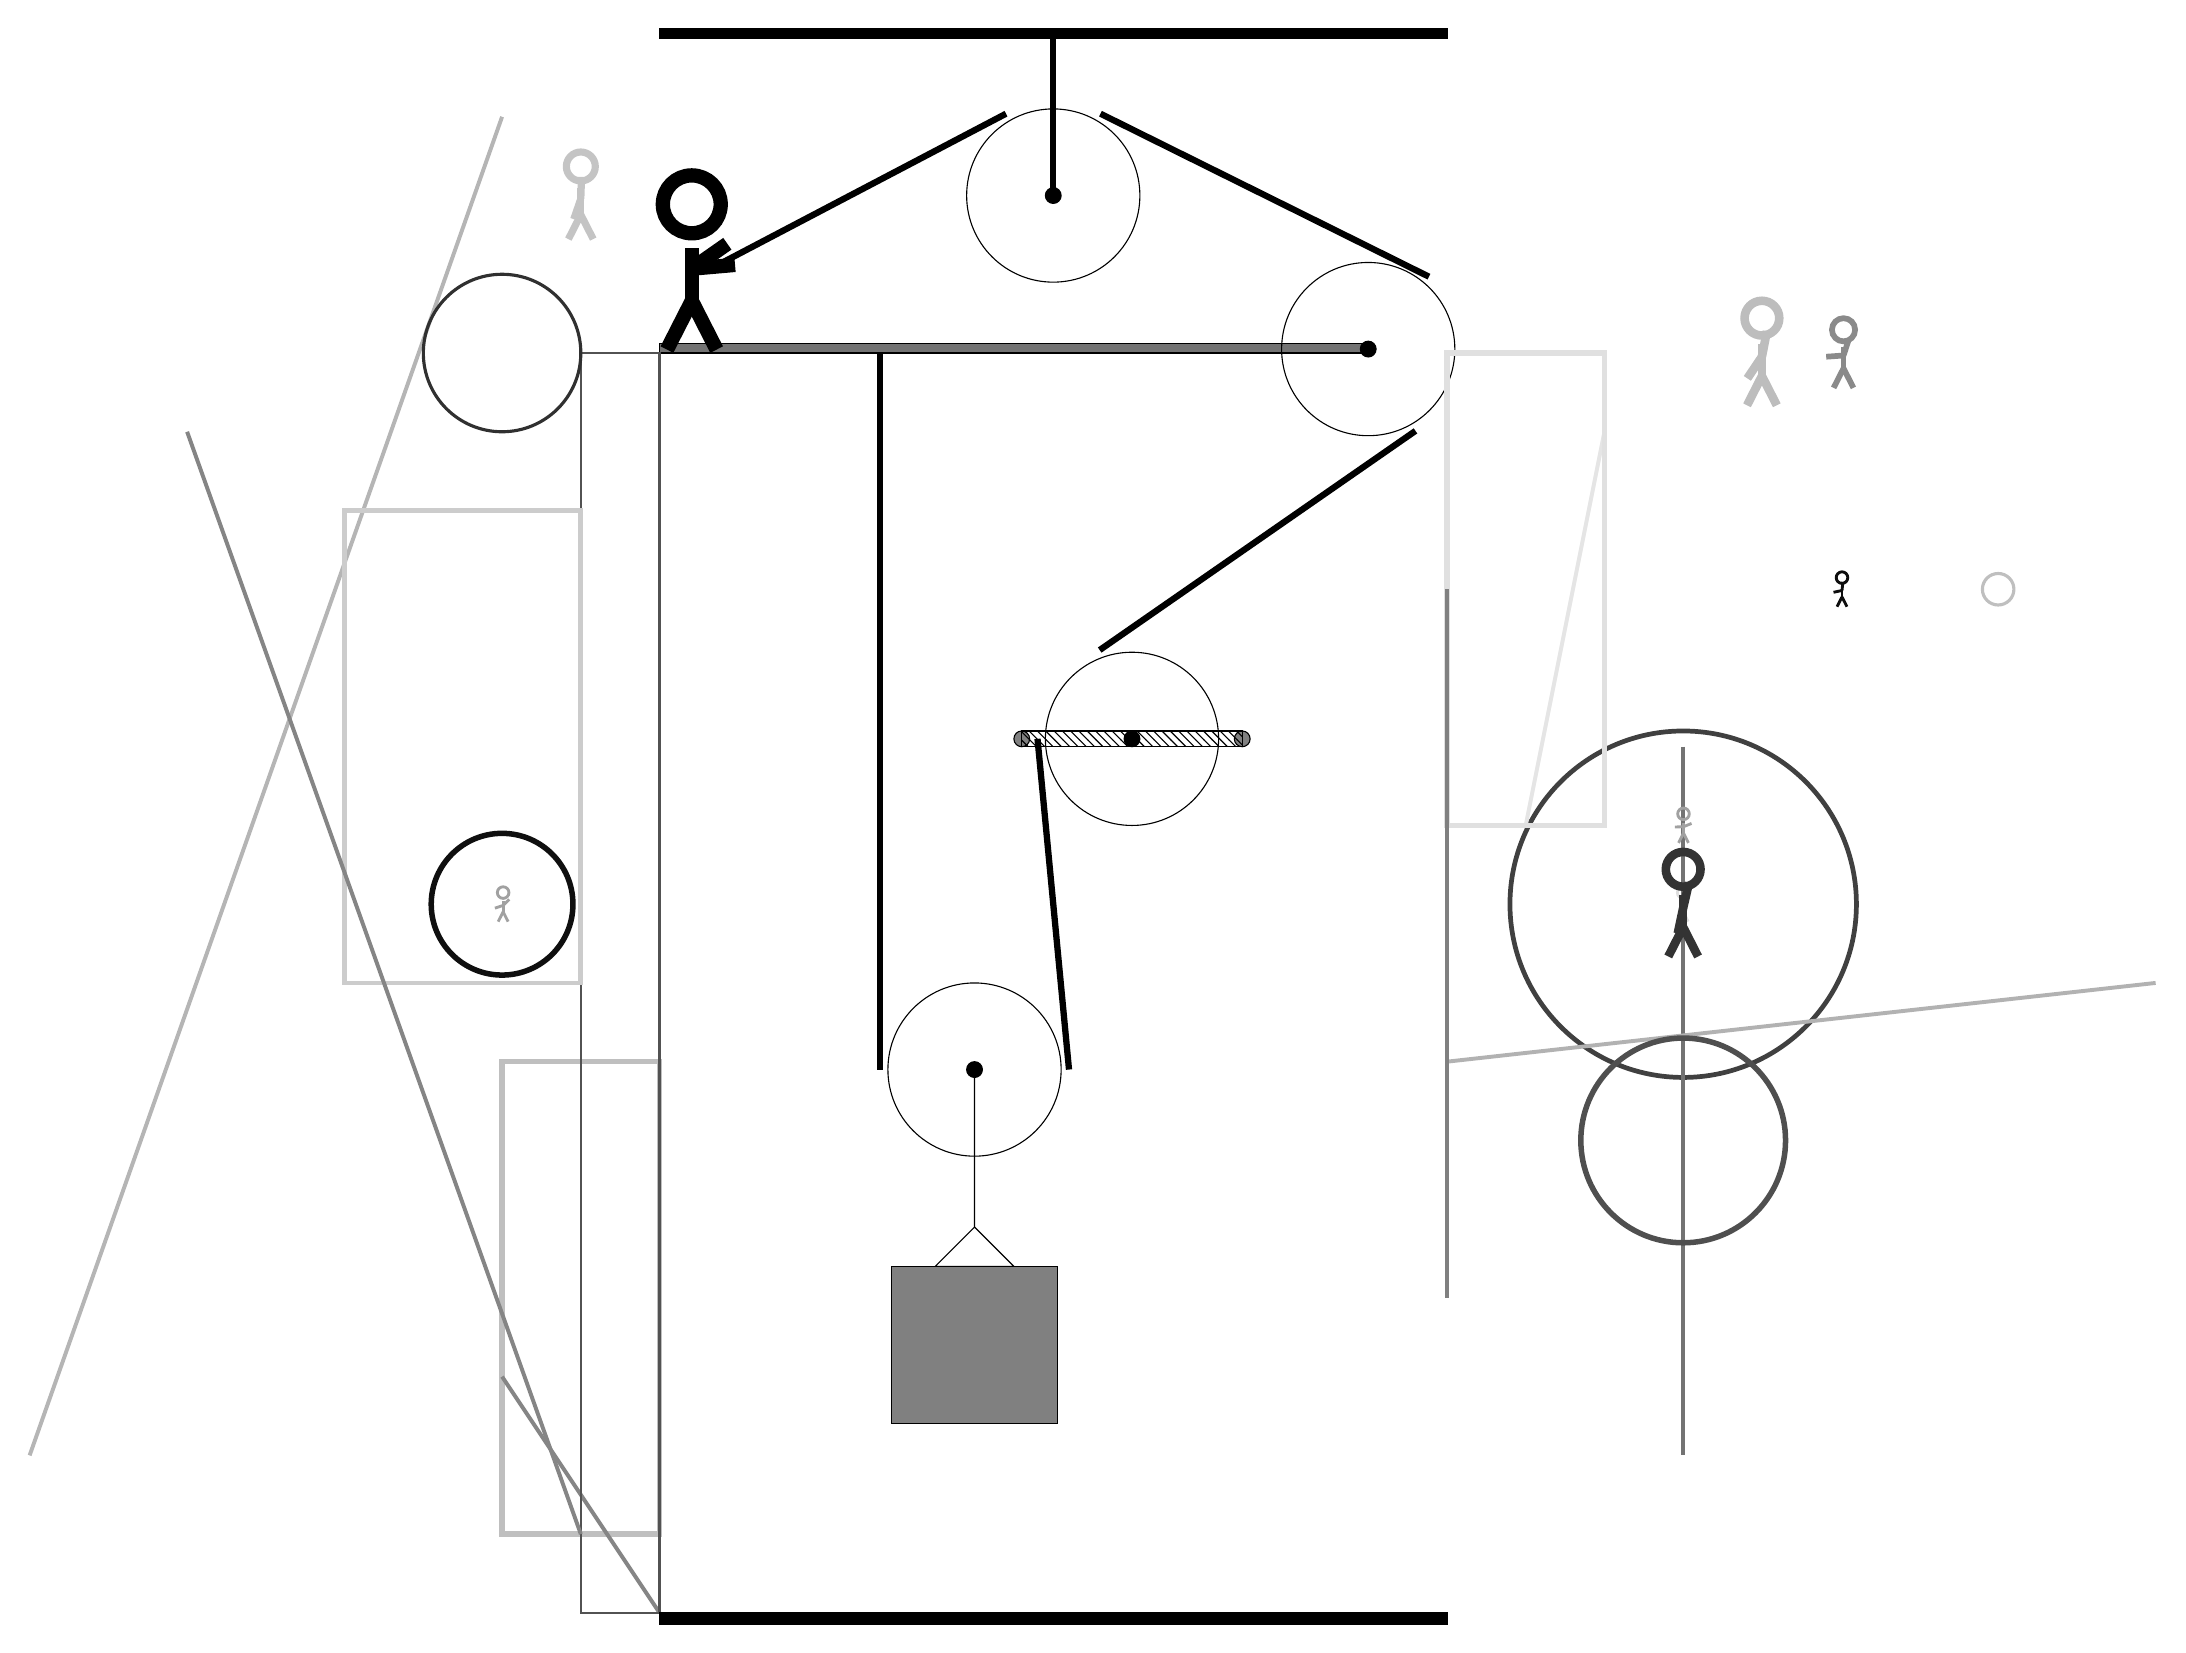
\begin{tikzpicture}
			%%%%% START %%%%%
			
			\draw[fill=black] (-2, 18) rectangle (8, 18.125);
			
			\draw[fill=black!55] (-2, 14) rectangle (7, 14.125);
			
			\draw (2, 4.9) circle (1.1);
			\draw[fill=black] (2, 4.9) circle (0.1);
			
			\draw (7, 14.05) circle (1.1);
			\draw[fill=black] (7, 14.05) circle (0.1);
			
			\draw[fill=white](4, 9.1) circle (1.1);
			\draw[fill=black] (4, 9.1) circle (0.1);
			\draw[fill=black!50] (2.6, 9.1) circle (0.1);
			\draw[fill=black!50] (5.4, 9.1) circle (0.1);
			\draw[pattern=north west lines, pattern color=black] (2.6, 9.2) rectangle (5.4, 9.0);
			
			\draw (3, 16) circle (1.1);
			\draw[fill=black] (3, 16) circle (0.1);
			\draw[line width=0.8mm] (3, 16) -- (3, 18);
			
			\draw (2, 4.9) -- (2, 2.9) -- (1.5, 2.4) -- (2.5, 2.4) -- (2, 2.9);
			\draw[fill=black!50] (0.95, 2.4) rectangle (3.05, 0.4);
			
			\draw[line width=0.8mm] (0.8, 14) -- (0.8, 4.9);
			\centerarc[line width=0.8mm](2, 4.9)(180:360:1.2000000000000002);
			\draw[line width=0.8mm](3.2, 4.9) -- (2.8, 9.1);
			\centerarc[line width=0.8mm](4, 9.1)(110:180:1.2000000000000002);
			\draw[line width=0.8mm](3.5896, 10.2276) -- (7.6, 13.0108);
			\centerarc[line width=0.8mm](7, 14.05)(-60:50:1.2000000000000002);
			\draw[line width=0.8mm](7.7714, 14.9692) -- (3.6, 17.0392);
			\centerarc[line width=0.8mm](3, 16)(60:120:1.2000000000000002);
			\draw[line width=0.8mm](2.4, 17.0392) -- (-1.2, 15.15);
			
			\node at (-1.5, 15.15) {\Strichmaxerl[10][-175][35]};
			
			\node[line width=0.7mm, color=black!46] at (13, 14) {\Strichmaxerl[4][4][72]};
			
			\node[line width=0.6mm, color=black!13] at (11, 7) {\Strichmaxerl[2][76][71]};
			\draw [line width=0.6mm, color=black!75](11, 7) circle (2.2);
			\draw[line width=0.5mm, color=black!55](11, 9) -- (11, 0);
			\draw[line width=0.7mm, color=black!25] (-2, 5) rectangle (-4, -1);
			\draw[line width=0.5mm, color=black!48](-2, -2) -- (-4, 1);
			\node[line width=0.7mm, color=black!26] at (12, 14) {\Strichmaxerl[6][56][79]};
			
			\draw [line width=0.7mm, color=black!94](-4, 7) circle (0.9);
			\draw[line width=0.3mm, color=black!68] (-2, 14) rectangle (-3, -2);
			
			\draw[line width=0.5mm, color=black!29](-4, 17) -- (-10, 0);
			
			\node[line width=0.4mm, color=black!37] at (11, 8) {\Strichmaxerl[2][2][22]};
			\draw [line width=0.4mm, color=black!81](-4, 14) circle (1.0);
			\draw[line width=0.5mm, color=black!10](10, 13) -- (9, 8);
			
			\draw[line width=0.7mm, color=black!12] (10, 14) rectangle (8, 8);
			\node[line width=0.3mm, color=black!80] at (11, 7) {\Strichmaxerl[6][78][77]};
			\node[line width=0.7mm, color=black!37] at (-4, 7) {\Strichmaxerl[2][18][45]};
			\draw[line width=0.5mm, color=black!30](8, 5) -- (17, 6);
			\draw [line width=0.7mm, color=black!69](11, 4) circle (1.3);
			\draw[line width=0.5mm, color=black!50] (8, 11) rectangle (8, 2);
			\node[line width=0.6mm, color=black!23] at (-3, 16) {\Strichmaxerl[5][71][88]};
			\node[line width=0.2mm, color=black!95] at (13, 11) {\Strichmaxerl[2][12][84]};
			\draw [line width=0.4mm, color=black!25](15, 11) circle (0.2);
			\draw[line width=0.6mm, color=black!20] (-3, 6) rectangle (-6, 12);
			\draw[line width=0.5mm, color=black!48](-3, -1) -- (-8, 13);
			
			\draw[fill=black] (-2, -2) rectangle (8, -2.15);
			
			%%%%% END %%%%%
		\end{tikzpicture}
	\end{figure}	
\end{document}